\section{Materials and Methods}
    
    \frame{\sectionpage}

    \begin{frame}{Trial Structure}
        \begin{figure}\label{fig:trial_structure}
        \centering
        \includegraphics[height = 0.65 \textheight]{images/fig.png}
        \caption{Program Timeline}
        \end{figure}
        
    \end{frame}

    \begin{frame}{\textit{Treatment:} The Anti-corruption Program in Brazil}
    
    \begin{columns}

    \begin{column}{0.5\textwidth}
        \begin{figure}\label{fig1}
        \centering
        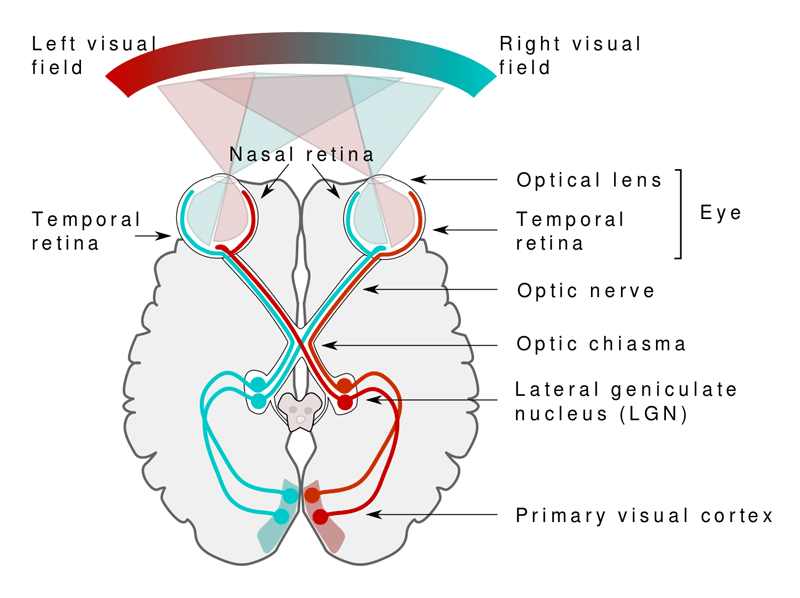
\includegraphics[height = 0.65 \textheight]{images/fig1.png}
        \caption{Program Timeline}
        \end{figure}
    \end{column}
    
    \begin{column}{0.4\textwidth}
    
    \begin{itemize}
      	\item<2-> sample: population \textbf<3->{\textcolor<3->{orange}{$<$450,000}}
      	\item<5-> selection by lottery
      	\item<6-> auditing process
      	\item<8-> audit report release
      \end{itemize}
    
    \only<3-4>{
    \begin{block}{\small \textbf{Important details}}
    \footnotesize
       \only<3-4>{\begin{itemize}
           \item<3-4> 92\% of all municipalities
           \item<3-4> 73\% of total population
           \item<4> excluding most state capitals/coastal cities
       \end{itemize}}
    \end{block}
    }
    
    \end{column}
    \end{columns}
    \end{frame}
    

    \begin{frame}{Technical details}
        \begin{itemize}
            \item<+-> Participants: 29 (\textcolor{lightlavender}{\textbf{normal/corrected-to-normal}} vision; age $24\pm 2.7$ years; 11 male, 18 female)
            \item<+-> Stimuli: projected at 120Hz onto
        \end{itemize}
        
    \end{frame}

    \begin{frame}{\textit{Information:} The Measure of Corruption}
    
    \only<1-7>{
    \underline{What information is revealed on the audit reports}?
    \begin{itemize}
        \item<2-> \textbf{\textcolor{orange}{Quantitative:}} total amount of federal funds  transferred and the amount audited
        \item<3->\textbf{\textcolor{orange}{Qualitative:}} an itemized list describing each irregularity
    \end{itemize}}
    
    \begin{columns}[T]

    \begin{column}{0.3\textwidth}
        \uncover<4->{\begin{block}{\small \centering \textbf{Irregular procurement}}
        \uncover<5->{\footnotesize
        \begin{itemize}
            \item[-] no call for bids or minimum number of bids not attained
            \item[-] evidence of fraud
        \end{itemize}
        }
        \end{block}}
    \end{column}
    
    \begin{column}{0.3\textwidth}
        \uncover<4->{\begin{block}{\small \centering \textbf{Diversion of public funds}}
        \uncover<6->{\footnotesize
        \begin{itemize}
            \item[-] expenditure without proof
            \item[-] direct evidence of diversion
        \end{itemize}
        }
        \end{block}}
    \end{column}
    
    \begin{column}{0.3\textwidth}
        \uncover<4->{\begin{block}{\small \centering \textbf{Over-invoicing}}
        \uncover<7->{\footnotesize
        \begin{itemize}
            \item[-] purchase of public goods and services above the market price
        \end{itemize}
        }
        \end{block}}
    \end{column}
    
    \end{columns}
    
    \only<8->{
    \vspace{15pt}
    \underline{Construct a single measure}: the \textbf<9>{\textcolor<9>{orange}{total number of times}} each one of the three irregularities appears
    \begin{itemize}
        \small
        \item<10-> \textbf{\color{orange}Justification 1}: most common
        \item<11-> \textbf{\color{orange}Justification 2}: often complementary
        \item<12> {\footnotesize My interpretation: Layer 1 measure of corruption magnitude, could be more detailed, quantitatively}
    \end{itemize}
    }
        
    \end{frame}
    